% Chapter 1
\chapter{مقدمه}

در سال‌های اخیر استفاده از انرژی‌های تجدید‌پذیر و جایگزین کردن آن‌ها به جای سوخت‌های فسیلی در کشور‌های توسعه‌یافته و صنعتی با رشد قابل توجهی همراه بوده است. یکی از این انرژی‌های تجدید‌پذیر که بیشتر از سایر انرژی‌ها مورد استفاده قرار گرفته است، انرژی باد است.  توربین‌های بادی طی دو مرحله انرژی باد را به انرژی الکتریکی تبدیل می‌کنند. در مرحله‌ی اول روتور توربین بادی انرژی جنبشی باد را به انرژی مکانیکی تبدیل می‌کند و در مرحله‌ی دوم انرژی مکانیکی توسط ژنراتور به انرژی الکتریکی تبدیل می‌شود. توربین‌های بادی سیستم‌های الکترومکانیکی پیچیده‌ای هستند و از این رو در معرض عیوب\LTRfootnote { Fault } متنوعی در قسمت‌های مختلف همچون سیستم‌ها، محرک‌ها و حس‌گر‌ها قرار می‌گیرند.

از طرف دیگر تشخیص نادرست و دیر‌هنگام این عیوب سبب می‌شود که عیوب در کل سیستم پخش شوند و حتی باعث خرابی\LTRfootnote{ Failure } و از کار‌افتادگی\LTRfootnote{ Downtime } در قسمت‌های مختلف توربین شوند. بنابراین نیازمند مکانیزم کنترلی هستیم که بتواند عیب را در لحظات ابتدایی ظهورش در سیستم شناسایی\LTRfootnote{ Identification } کند و به جبران اثرات منفی عیب بپردازد. از آنجایی که استفاده از توربین‌های بادی در سال‌های اخیر پیشرفت چشمگیری داشته است، بر روی موضوعات مرتبط با توربین‌های بادی کارهای زیادی انجام گرفته است. در زمینه‌ی  آشکارسازی عیوب\LTRfootnote{ Fault Detection } و جداسازی\LTRfootnote{ Fault Isolation } آن‌ها مطالعات زیادی صورت گرفته و روش‌های متعددی ارائه شده است \cite{b6}. همچنین برای جبران اثرات عیب، روش‌های سازش با  عیب\LTRfootnote{  Fault Accomodation  } زیادی پیشنهاد شده‌اند.
\section{پیشینه تحقیق}
 
 \begin{figure}[t]
 \centering
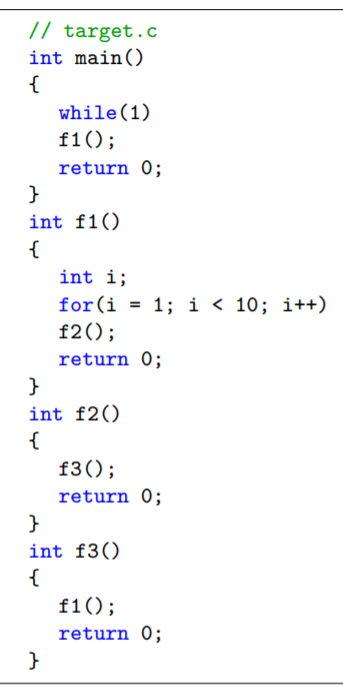
\includegraphics[height=8cm,width=10cm]{b.png}
\caption{ توربین بادی 12 کیلو‌وات (ساخته‌شده به وسیله‌ی چارلز فرانسیس براش) \cite{b1}.}
\label{wt}
\centering
\end{figure}

یک نمونه از توربین‌های بادی اولیه در شکل~\ref{wt} نشان داده شده است. در \cite{a1}، یک مدل معیار\LTRfootnote{ Benchmark Model } برای پیاده‌سازی و مقایسه‌ی روش‌های تشخیص و جداسازی عیب در توربین‌های بادی ارائه شده است. این مدل معیار، یک توربین بادی سه پره‌ی  محور افقی با سرعت متغیر و توان مجاز 4/8 مگا‌وات را که به کنترل گام\LTRfootnote{ Pitch Control }(تغییر زاویه‌ی پره‌‌های توربین بادی حول محور طولی پره‌ها با اعمال فرامین کنترلی) نیز مجهز است، شبیه‌سازی می‌کند. هدف از ارائه‌ی این مدل، بوجود آوردن یک فضای مناسب برای مقایسه و آزمایش روش‌های مختلف تشخیص و جداسازی عیوب بر روی توربین است. از این مدل می‌توان برای مقایسه‌ی روش‌های سازش با عیب که در زمینه‌ی توربین بادی ارائه شده‌اند، استفاده کرد. تعداد زیادی از تحقیقاتی که در سال‌های گذشته در زمینه‌ی تشخیص و جداسازی عیب و همچنین سازش با عیب انجام گرفته است، طرح‌های پیشنهادی خود را بر روی این مدل آزمایش و مقایسه کرده‌اند. 

یکی از اجزای توربین بادی که در معرض عیب قرار دارد، محرک گام پره‌ی توربین می‌باشد. هر یک از پره‌های توربین بادی توسط یک محرک کنترل می‌شوند و با وقوع عیب در  محرک‌ گام هر پره، موقعیت گام آن پره با خطای زیادی مواجه می‌شود. برای حل این مساله،  در \cite{a10} یک روش جبران مبتنی بر تخصیص کنترل\LTRfootnote{ Control Allocation } ارائه شده است. تخصیص کنترل، یکی از رایج‌ترین روش‌های کنترل انعطاف‌پذیر در برابر عیب است. در روش پیشنهادی، گشتاوری که بر اثر عیب یکی از محرک‌ها اتلاف می‌شود، توسط اعمال قانون کنترلی به دو محرک دیگر جبران می‌گردد و توان مطلوب توربین بادی قابل دست‌یابی است.



\section{اهداف و دستاوردهای تحقیق}
از آنجایی که کنترل‌کننده‌ی توربین بادی برای تعیین ناحیه‌ی کنترلی و اعمال دستورات کنترلی مناسب، از اطلاعات حاصل از حس‌گر‌ها استفاده می‌کند؛ وقوع عیب در حس‌گر‌ها می‌تواند سبب تغذیه‌ی اشتباه کنترل‌کننده‌ی توربین شود. در صورتی که کنترل‌کننده‌ی توربین از اطلاعات اشتباه حس‌گر‌ها استفاده کند، دستورات کنترلی که به محرک‌ها اعمال می‌کند اشتباه خواهند بود. این امر سبب می‌شود تا با گذشت زمان، کل سیستم تحت تاثیر قرار گرفته و از حالت بدون عیب فاصله بگیرند. 

در این پایان‌نامه، طرحی پیشنهاد شده است که باعث جلوگیری از کاهش راندمان سیستم، در صورت وجود عیب در حس‌گر‌های اطراف پیشرانه‌ی توربین بادی خواهد شد. در این تحقیق، تشخیص زمان و مکان وقوع عیب، شدت عیب و جداسازی عیب‌ها از یکدیگر به صورت آنلاین مورد بررسی قرار گرفته است. با فرض این که حس‌گر‌های سرعت روتور و ژنراتور و همچنین گشتاور ژنراتور (حس‌گر‌های اطراف پیشرانه‌ی توربین بادی) دچار عیب شوند، با مدل‌سازی مناسب پیشرانه، رویتگر‌هایی را برای تخمین حالت و تولید مانده طراحی کرده و با کمک این رویتگر‌ها (که از نوع رویتگر‌های ورودی ناشناخته هستند)، برای هر یک از حس‌گر‌ها به طور جداگانه سیگنال آشکارسازی عیب تولید می‌کنیم. 

آشکارسازی آنلاین  و سازش با عیوب حس‌گر که در این پایان‌نامه ارائه شده است، بر روی مدل معیار توربین بادی پیاده‌سازی شده و با روش‌های دیگر مورد مقایسه قرار گرفته است. نتایج شبیه‌سازی، بهبود عملکرد سیستم را در صورت بکار‌گیری روش پیشنهادی نشان خواهد داد. 


\section{ساختار پایان‌نامه}
در فصل دوم  به طور مختصر با تاریخچه‌ی انرژی باد آشنا خواهیم شد. همچنین نحوه‌ی عملکرد توربین بادی و اجزای تشکیل‌دهنده‌ی توربین را نیز در این فصل بررسی خواهیم کرد. در پایان این فصل با انواع تقسیم‌بندی‌های توربین‌های بادی از نظر مکان نصب و نحوه‌ی اتصال به شبکه و قرار‌گیری روتور توربین به طور مختصر آشنا خواهیم شد.

در فصل پایانی به بیان نتایج پایان‌نامه و ارائه چند پیشنهاد پرداخته خواهد شد. 

